\documentclass{article} % For LaTeX2e
\usepackage{iclr2026_conference,times}

\input{math_commands.tex}

\usepackage{hyperref}
\usepackage{url}
\usepackage{graphicx}
\usepackage{booktabs}

\title{What Do Sequential Generative Latents Encode?\\
Probing a DreamerV3 World Model Against a Static VAE}

\author{Ricky (Xinrui) Bao \\
University of Chicago \\
\texttt{rickybao@uchicago.edu}}

\newcommand{\rtwo}{$R^2$}
\iclrfinalcopy

\begin{document}

\maketitle

\begin{abstract}
World models such as DreamerV3 learn a sequential generative latent by training
a recurrent latent-dynamics model on streams of observations. Unsupervised
representation learning, by contrast, is usually studied on static data. We ask
what the sequential latent encodes that a static, per-frame model does not. We
freeze a DreamerV3 recurrent state-space model (RSSM) and a static frame-level
variational autoencoder (VAE) trained on the same DeepMind Control
proprioceptive Walker-Walk observation stream, then probe both with held-out
ridge and MLP regression across three axes: the probe target (current or future
simulator state, and derived dynamical quantities), the probe site (encoder,
RSSM posterior, RSSM prior, VAE latent), and the temporal receptive field given
to the static model. We find that (i) per-frame current state is decoded equally
well by both models, and the RSSM's small edge lies in its deterministic state
rather than its categorical stochastic latent; (ii) a static VAE allowed to see
a few past frames matches or exceeds the RSSM at current-state decoding; (iii)
the sequential latent's main, dimension-independent advantages are a cyclic
dynamical quantity (gait phase, $+0.21$ \rtwo) and action-conditioned future
prediction through the learned prior ($R^2\approx0.50$ at a 20-step horizon
versus $0.16$ for static extrapolation); and (iv) generative likelihood and
probe \rtwo{} decouple, with reconstruction improving as capacity and training
grow while linearly decodable state content saturates.
\end{abstract}

\section{Introduction}

A world model is a learned representation of states that can be rolled forward
to predict future states \citep{ha2018worldmodels}. DreamerV3
\citep{hafner2025dreamerv3} instantiates this with a recurrent state-space model
(RSSM) \citep{hafner2019planet}: an observation is encoded into a stochastic
latent that is concatenated with a deterministic recurrent state, and the model
is trained to reconstruct observations and to predict its own next latent. The
resulting representation is sequential, shaped by temporal context and a learned
transition model. Most unsupervised representation learning, by contrast, is
developed and analyzed on static data, for example a VAE \citep{kingma2014vae}
over images. This motivates a concrete question: what does a sequential
generative latent encode beyond what a static, per-frame model extracts from the
same observations?

We answer this empirically with a controlled comparison. We freeze a trained
DreamerV3 RSSM and a static frame-level VAE trained on the identical observation
stream, and evaluate both with a probing battery that fits simple readout
functions on the frozen features and measures held-out predictive accuracy
\citep{alain2016probes}. To make ``static versus sequential'' an empirical
contrast rather than an assumption, the VAE reuses DreamerV3's exact encoder, a
matched decoder, and the same observation model, so that the only difference is
the absence of recurrence and learned dynamics.

\textbf{Contributions.} (1) A controlled VAE-versus-RSSM comparison that shares
encoder, decoder, observation model, and training data, isolating sequential
structure. (2) A three-axis probing battery (probe target, probe site including
the RSSM prior and open-loop imagination, and temporal receptive field),
together with held-out generative likelihood. (3) Four findings
(\S\ref{sec:results}): per-frame content is shared, static aggregation closes the
current-state gap, the sequential latent's advantage is predictive and
dynamical, and generative quality decouples from probe quality. (4) A fully
reproducible pipeline.\footnote{Code: \texttt{probing/} in the project
repository; figures are regenerated by \texttt{result\_images/build\_summary\_figures.py}.}

\section{Background and setup}
\label{sec:setup}

\paragraph{RSSM world model.} At each step $t$ the RSSM maintains a
deterministic recurrent state $h_t=f_\phi(h_{t-1},z_{t-1},a_{t-1})$ and a
stochastic latent with a posterior $z_t\sim q_\phi(z_t\mid h_t,x_t)$ that sees
the observation $x_t$ and a prior $\hat z_t\sim p_\phi(\hat z_t\mid h_t)$ that
does not. The model state is $s_t=(h_t,z_t)$ and a decoder reconstructs
$\hat x_t=d_\phi(s_t)$. In our configuration $z_t$ is a set of $32$ categorical
variables with $4$ classes each ($128$ dimensions), and $h_t$ has $512$
dimensions. The model is trained with reconstruction and a KL term that aligns
posterior and prior \citep{hafner2025dreamerv3}.

\paragraph{Static VAE.} Our baseline removes the recurrence and dynamics while
holding everything else fixed. It uses DreamerV3's encoder $e_\phi$ to map a
single frame $x_t$ to a diagonal-Gaussian latent $q(z\mid x_t)=\mathcal{N}(\mu(x_t),
\mathrm{diag}\,\sigma^2(x_t))$, and a decoder matched to the RSSM's vector
decoder. It is trained on the per-frame objective
\begin{equation}
\mathcal{L}_\beta(x) = \underbrace{\E_{q(z\mid x)}\!\big[-\log p(x\mid z)\big]}_{\text{reconstruction}}
\;+\; \beta\,\KL\!\big(q(z\mid x)\,\Vert\,\mathcal{N}(0,I)\big),
\label{eq:elbo}
\end{equation}
the (negative) evidence lower bound for $\beta{=}1$ \citep{kingma2014vae,
higgins2017betavae}, optimized with the reparameterization $z=\mu+\sigma\odot
\epsilon$. Both models use the same observation model, a unit-variance Gaussian
in $\mathrm{symlog}$ space, $\mathrm{symlog}(x)=\mathrm{sign}(x)\log(1+|x|)$, so
that $-\log p(x\mid z)=\tfrac12\Vert\mathrm{symlog}(x)-d(z)\Vert^2+\text{const}$
and held-out log-likelihoods are computed identically. We set the VAE latent to
$128$ dimensions to match the RSSM's stochastic latent. Because encoder,
decoder, observation model, and training frames are shared, any probe gap is
attributable to sequential structure rather than architecture.

\paragraph{Task, models, and data.} We use DeepMind Control
\citep{tassa2018dmc} Walker-Walk with proprioceptive observations
(\texttt{orientations}, \texttt{height}, \texttt{velocity}). We train three
DreamerV3 seeds and one VAE per seed on that seed's replay buffer. Two seeds are
trained to $500$K environment steps and one to $1.1$M; the longer run is treated
as an auxiliary point rather than pooled, and we report per-seed values with the
matched $500$K pair as the spread, since the training-length difference affects
generative likelihood but not probe \rtwo{} (\S\ref{sec:gen}). Probe trajectories
are $40$ held-out episodes ($1000$ steps) rolled out from the frozen evaluation
policy, logging the full MuJoCo physics state ($q_{\text{pos}}\,|\,q_{\text{vel}}$),
which the replay buffer does not store.

\section{Probing methodology}
\label{sec:method}

For a frozen representation $z$ and a target $y$ we fit a probe $g$ and report
the held-out coefficient of determination
\begin{equation}
R^2 = 1 - \frac{\sum (y-g(z))^2}{\sum (y-\bar y_{\text{train}})^2},
\end{equation}
against the train-set mean baseline, so an uninformative representation scores
$\approx 0$ and negative values are possible on held-out episodes. The probe
family is fixed across all sites and targets, namely a closed-form ridge
regressor (regularization chosen on a validation split of the training episodes)
and a small two-hidden-layer MLP, so differences reflect the representation
rather than the probe. Train and test splits are by episode. We vary three axes:
\begin{itemize}
\item \textbf{Probe target:} the current simulator state; the future state at
horizon $k\in\{1,5,20\}$; and derived dynamical quantities (gait phase, encoded
as $(\cos,\sin)$ of the analytic-signal phase of the antiphase hip oscillation;
discounted return-to-go; time-to-fall).
\item \textbf{Probe site:} encoder output; RSSM posterior ($h_t$ and $\mathbb{E}[z_t]$,
also probed separately); RSSM prior, both one-step and open-loop $k$-step
(roll the prior forward with the recorded actions and probe the imagined state);
VAE encoder output; VAE latent mean.
\item \textbf{Receptive field:} the VAE latent given $1$, $4$, $16$ or all past
frames (a causal concatenation), measuring how much sequential content a static
model recovers by post-hoc temporal aggregation.
\end{itemize}
We additionally report held-out reconstruction and one-step predictive
log-likelihood, computed identically for both models (\S\ref{sec:setup}).

\section{Results}
\label{sec:results}

\begin{figure}[t]
\centering
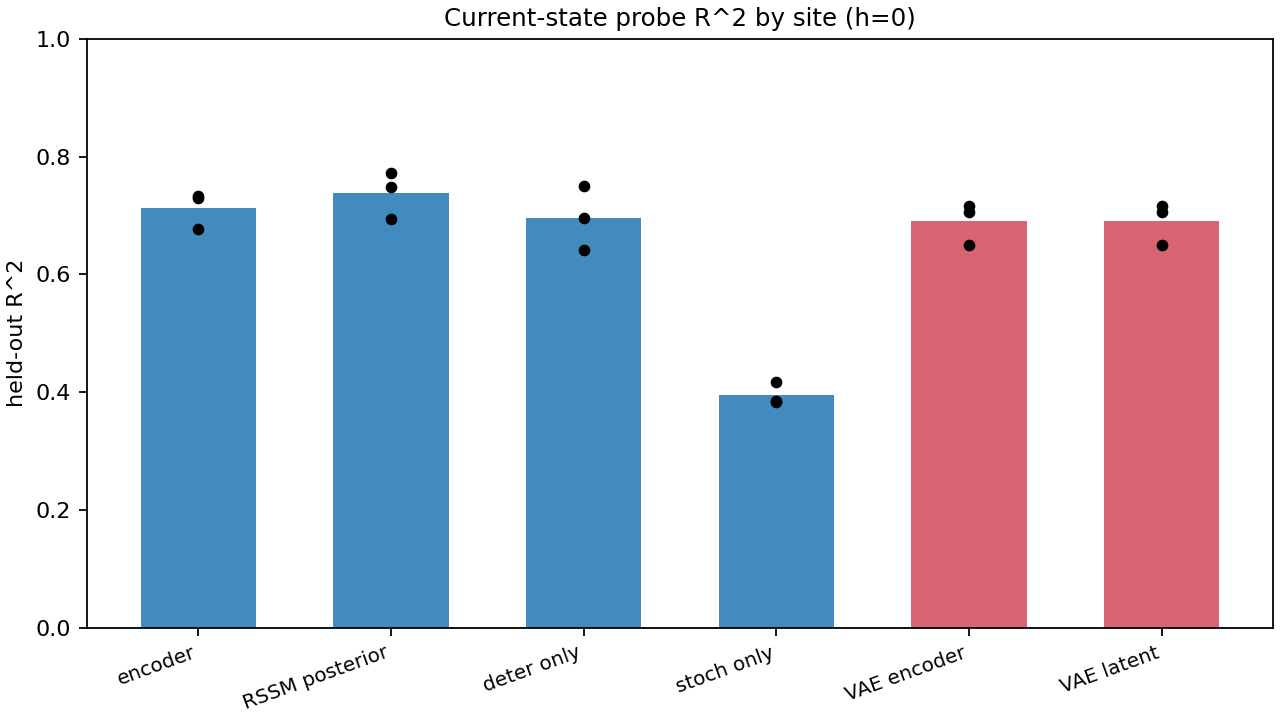
\includegraphics[width=0.49\textwidth]{figures/current_state_probe_r2_by_site.png}
\hfill

\includegraphics[width=0.49\textwidth]{figures/future_state_r2_by_horizon_posterior_vs_prior.png}
\caption{Held-out probe \rtwo{} (black dots are the three seeds; bars and lines
are the mean). \textbf{Left:} current simulator state ($h{=}0$) is decoded
equally well by the encoder, RSSM posterior, RSSM deterministic state, and the
VAE ($\approx0.7$); the categorical stochastic latent alone is a poor linear
code ($\approx0.40$). \textbf{Right:} a linear readout of future state from the
posterior decays quickly, whereas rolling the action-conditioned prior forward
(open-loop imagination) retains far more future-state information.}
\label{fig:probes}
\end{figure}

\subsection{Per-frame current state is shared; the RSSM edge is in $h_t$, not $z_t$}
Figure~\ref{fig:probes} (left) shows that the encoder, RSSM posterior, RSSM
deterministic state, VAE encoder, and VAE latent all decode the current state at
$R^2\approx0.69$ to $0.74$. The posterior's $+0.05$ over the VAE comes entirely
from its $512$-dimensional deterministic state ($R^2\approx0.70$); the
categorical stochastic latent alone scores only $\approx0.40$. At equal width
($128$), the continuous VAE latent ($0.69$) is a stronger linear state code than
the RSSM's categorical latent ($0.40$). The RSSM therefore leads at $h{=}0$ only
because it carries a larger deterministic state, not because the generative
latent is intrinsically richer per frame.

\subsection{The world model's advantage is predictive}
A linear readout of future state from the posterior decays sharply with horizon
($R^2 = 0.74,\,0.50,\,0.30,\,0.16$ at $k=0,1,5,20$; Figure~\ref{fig:probes},
right). Rolling the prior forward with the recorded actions and probing the
imagined state retains much more information ($R^2 = 0.72,\,0.66,\,0.50$ at
$k=1,5,20$). At a $20$-step horizon the action-conditioned prior reaches
$\approx0.50$ versus $0.16$ for static extrapolation, roughly three times the
future-state content. This is the clearest advantage of the sequential model:
its learned dynamics, not a static readout of the current latent, carry the
future. Appendix Figure~\ref{fig:openloop} visualizes a single open-loop rollout
and the prediction error growing with horizon.

\begin{figure}[t]
\centering
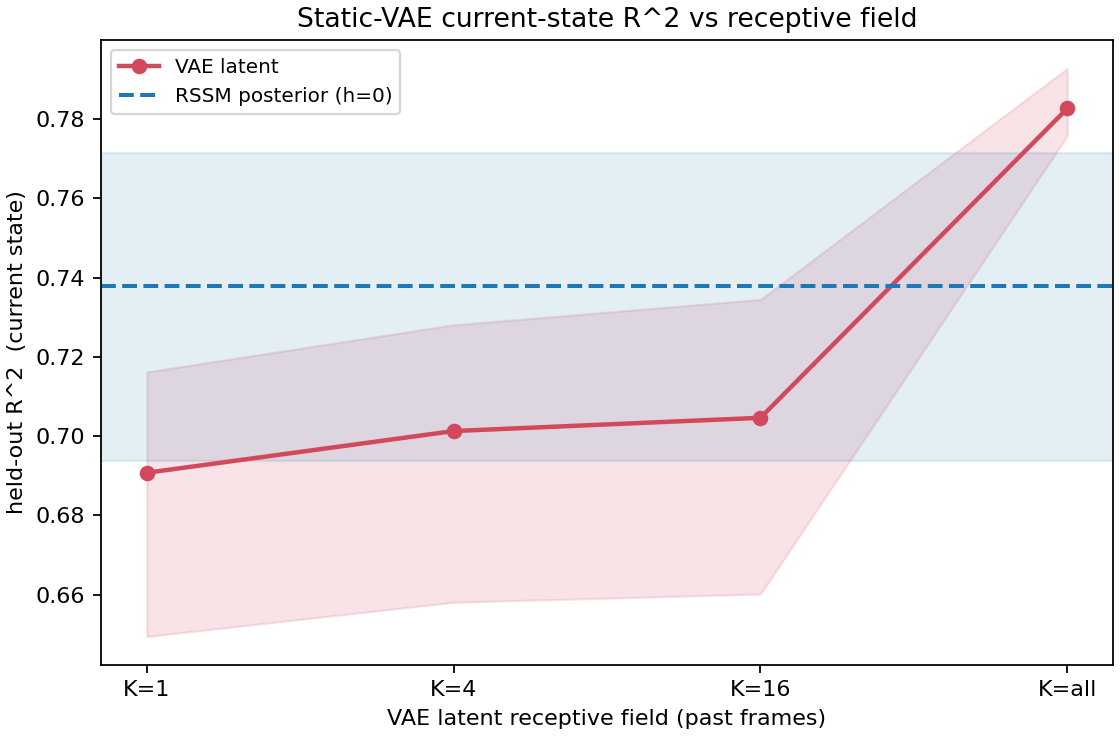
\includegraphics[width=0.49\textwidth]{figures/vae_receptive_field_r2.png}
\hfill
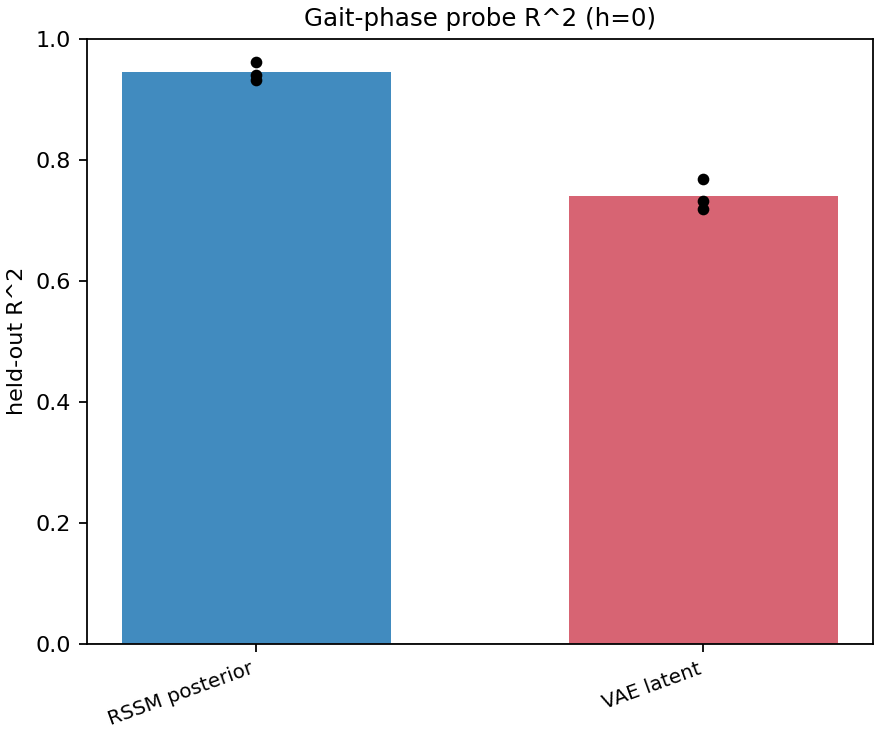
\includegraphics[width=0.49\textwidth]{figures/gait_phase_r2_rssm_vs_vae.png}
\caption{\textbf{Left:} the static VAE's current-state \rtwo{} rises with its
temporal receptive field and overtakes the RSSM posterior reference once it sees
all past frames; recurrence adds little for current-state decoding that simple
aggregation cannot recover. \textbf{Right:} gait phase, a cyclic dynamical
quantity, is decoded markedly better by the recurrent posterior than by the
single-frame VAE latent.}
\label{fig:gap}
\end{figure}

\subsection{A static model recovers the current-state gap by aggregating frames}
Figure~\ref{fig:gap} (left) shows the VAE latent's current-state \rtwo{} rising
from $0.69$ (one frame) to $0.78$ at all past frames, overtaking the RSSM
posterior ($0.74$). For current observable state, recurrence supplies
essentially nothing that post-hoc temporal aggregation of static features cannot
reproduce. The sequential representation's value is not in richer current-state
encoding.

\subsection{Gait phase: a dynamical quantity that favors the RSSM}
Figure~\ref{fig:gap} (right) shows the one place a low-dimensional,
dimension-independent target favors the RSSM decisively: gait phase is decoded at
$R^2\approx0.95$ from the posterior versus $\approx0.74$ from the VAE latent
($+0.21$, consistent across all three seeds). Phase is inherently about position
within a cycle, which a single frame cannot disambiguate; the recurrent latent
encodes it, the static one does not. (Return-to-go is near-zero for both models,
and time-to-fall is unreliable due to censoring, since a competent walker rarely
falls; see Appendix~\ref{app:nulls}.)

\subsection{Generative quality and probe quality decouple}
\label{sec:gen}
Table~\ref{tab:nll} reports held-out negative log-likelihood. The RSSM
reconstructs the current frame with much lower NLL than the VAE (and better on
$90$ to $97\%$ of frames), and its NLL drops sharply from $500$K to $1.1$M
training steps (seed~0: $0.36$; seeds~1 and~2: $0.67$ and $0.62$). Yet its
current-state probe \rtwo{} is within seed noise of the others
(Figure~\ref{fig:probes}, left). Thus better reconstruction does not yield
proportionally more linearly decodable state: generative fidelity improves with
capacity and training well past the point where probe content saturates. The two
metrics agree only partially, a caution against using either alone as a proxy for
representation quality.

\begin{table}[t]
\caption{Held-out NLL (lower is better), mean over the held-out probe set,
per seed (training steps in parentheses). The RSSM reconstructs and predicts far
better than the VAE, and improves strongly with training length, while
current-state probe \rtwo{} (Fig.~\ref{fig:probes}) stays flat, illustrating the
decoupling of generative and probe quality.}
\label{tab:nll}
\begin{center}
\begin{tabular}{lccc}
\toprule
Held-out NLL & seed 0 (1.1M) & seed 1 (500K) & seed 2 (500K) \\
\midrule
RSSM posterior reconstruction & 0.36 & 0.67 & 0.62 \\
RSSM prior one-step prediction & 0.80 & 1.78 & 1.47 \\
Static VAE reconstruction      & 1.58 & 1.95 & 1.77 \\
\bottomrule
\end{tabular}
\end{center}
\end{table}

\section{Discussion}

Across a controlled comparison that shares everything but recurrence, the
sequential generative latent does not encode more about the current observable
state than a static VAE; frame-stacking the static model matches it. Its
advantages are (1) cyclic and dynamical structure (gait phase) and (2)
action-conditioned future state through its learned prior, which predicts
$20$ steps ahead far better than a static extrapolation. Separately, generative
fidelity improves with capacity and training while linear state-decodability
saturates, so reconstruction likelihood and probe \rtwo{} should not be treated
as interchangeable measures of representation quality.

\textbf{Limitations.} We study one domain (Walker), one observation modality
(proprioception, where the current state is nearly fully observed from a single
frame), and one model size; the small per-frame gap may partly reflect this near
full observability. Probe \rtwo{} lower-bounds decodable information under a fixed
probe family and is not mutual information. Comparisons of the $640$-dimensional
posterior against the $128$-dimensional VAE latent are confounded by
dimensionality, which is why we also report the matched-width stochastic-latent
and deterministic-state probes. Finally, we have three seeds with one trained
longer, and therefore report per-seed values rather than a single pooled mean.

\subsubsection*{Acknowledgments}
Built on the open-source DreamerV3 implementation \citep{hafner2025dreamerv3}.
Compute was provided by the UChicago Research Computing Center.

\bibliography{references}
\bibliographystyle{iclr2026_conference}

\appendix
\section{Open-loop prediction}
\label{app:openloop}
Figure~\ref{fig:openloop} shows a representative open-loop rollout (seed~0): a
$25$-step posterior context followed by $75$ steps of prior imagination using the
recorded actions, decoded back to observation units. The posterior tracks the
truth closely; the prior then carries the gait oscillations forward for many
steps before gradually drifting, and the pooled prediction RMSE grows smoothly
with horizon.

\begin{figure}[h]
\centering
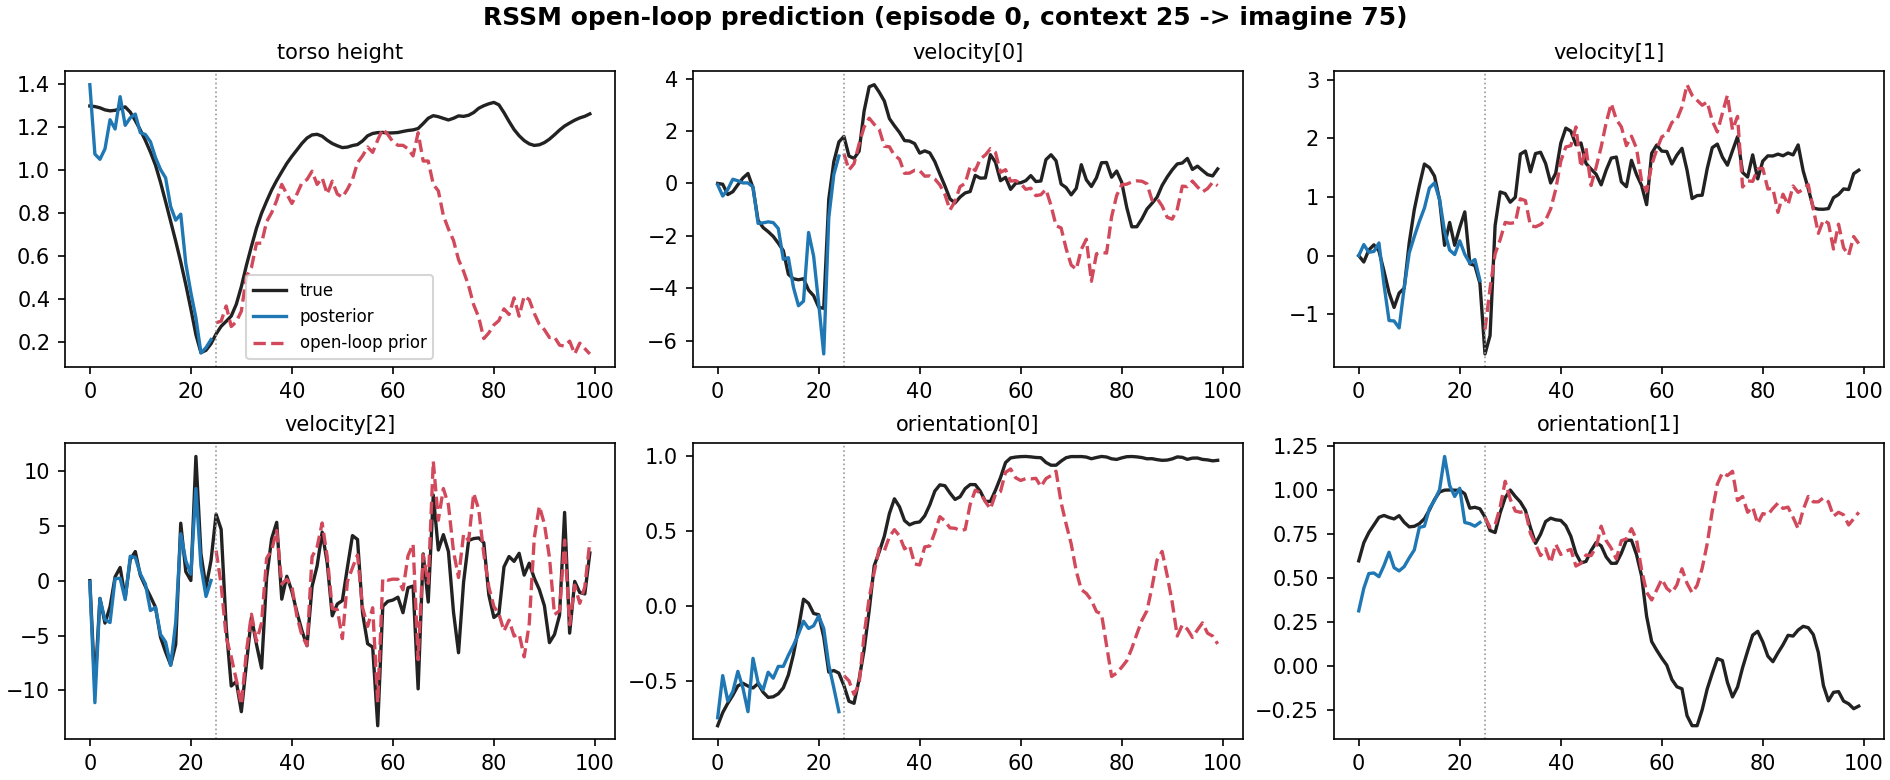
\includegraphics[width=0.62\textwidth]{figures/openloop_example_trajectory_seed0.png}
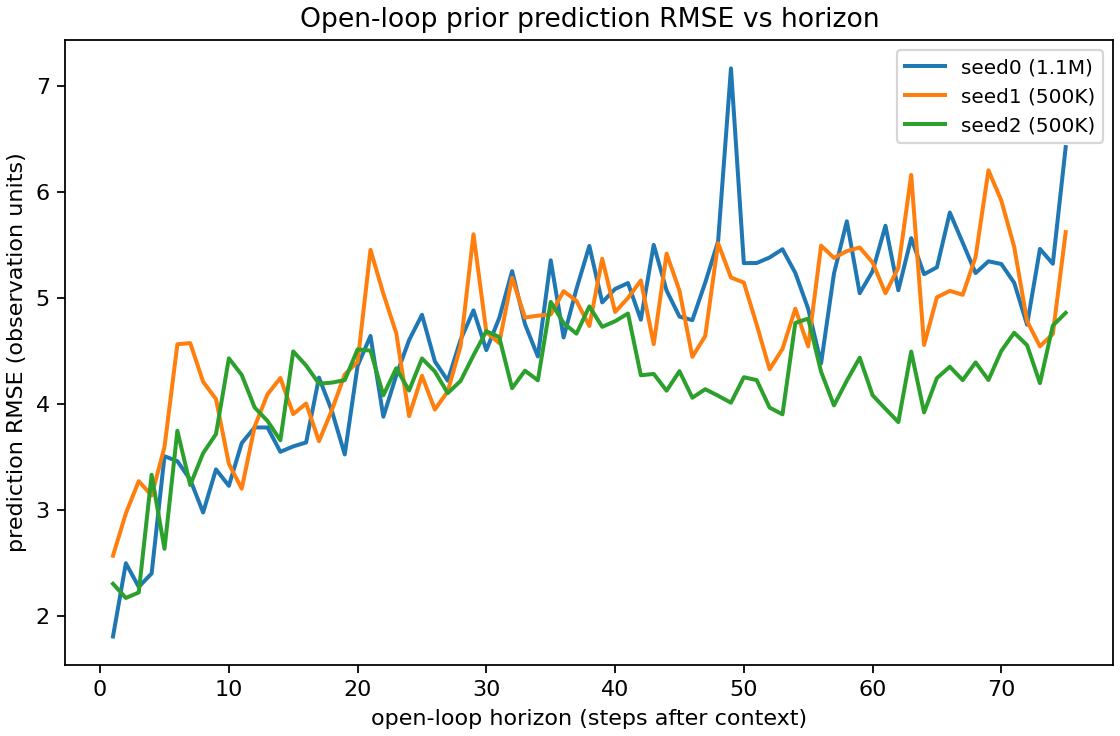
\includegraphics[width=0.36\textwidth]{figures/openloop_prediction_rmse_vs_horizon.png}
\caption{Open-loop prediction. Left: true (black), posterior reconstruction
(solid), open-loop prior prediction (dashed) per observation variable. Right:
pooled open-loop prediction RMSE versus horizon, per seed.}
\label{fig:openloop}
\end{figure}

\section{Generative quality and reconstruction advantage}
Figure~\ref{fig:gen} is the visual companion to Table~\ref{tab:nll}: held-out NLL
by quantity and seed (left), and the fraction of frames on which the RSSM
reconstructs better than the VAE (right).

\begin{figure}[h]
\centering
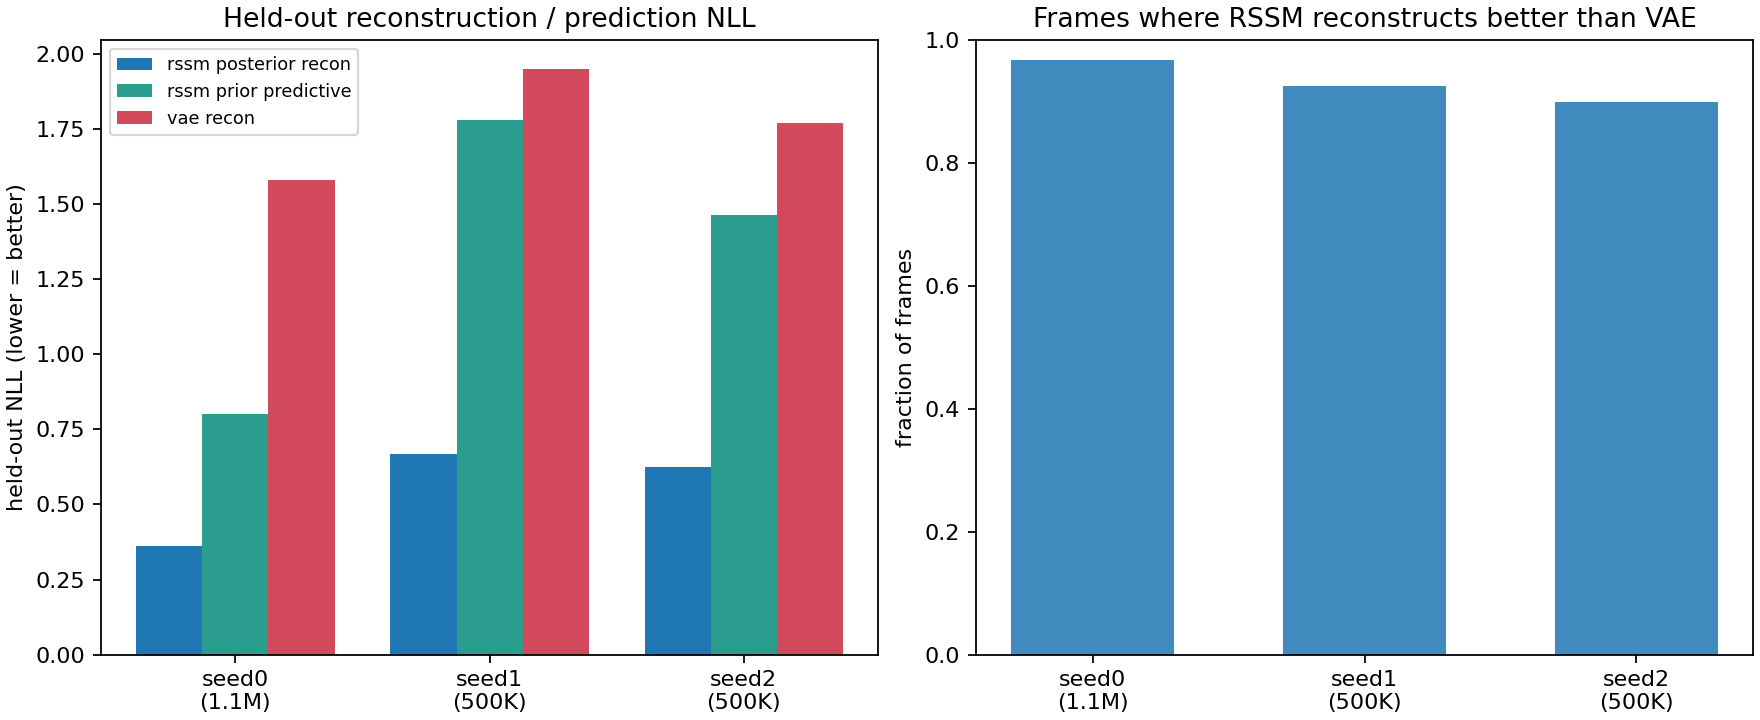
\includegraphics[width=0.9\textwidth]{figures/generative_nll_and_reconstruction_advantage.png}
\caption{Held-out reconstruction and prediction NLL (left) and the fraction of
frames where the RSSM reconstructs better than the VAE (right). Seed~0 ($1.1$M
steps) has much lower NLL than the $500$K seeds, while its probe \rtwo{} does not
correspondingly increase.}
\label{fig:gen}
\end{figure}

\section{Null and unreliable targets}
\label{app:nulls}
Two derived targets are reported for completeness but excluded from the main
findings. Return-to-go (discounted future reward) has near-zero \rtwo{} for both
models ($\approx-0.01$ posterior, $\approx0$ VAE) on Walker-Walk, where per-step
reward is nearly constant and not linearly decodable. Time-to-fall is highly
seed-dependent (posterior \rtwo{} of $0.06$, $0.50$, and $0.98$ across seeds)
because a competent walker rarely falls, so the target is dominated by rare,
heavily right-censored events; we therefore do not draw conclusions from it.

\section{Reproducibility details}
DreamerV3 uses the \texttt{dmc\_proprio}/\texttt{size1m} configuration
($h_t\in\mathbb{R}^{512}$, $z_t$ a set of $32{\times}4$ categoricals,
encoder and decoder MLPs of width $64$, depth $3$, symlog preprocessing). The
VAE shares the encoder and a matched decoder, with a $128$-dimensional Gaussian
latent, $\beta{=}1$, trained for $60$K steps (Adam, lr $3\times10^{-4}$) on each
seed's replay buffer. Probes use ridge (regularization selected on a validation
split) and a two-hidden-layer, width-$256$ ReLU MLP. The probe set is $40$ held-out
episodes of $1000$ steps from the frozen evaluation policy with logged physics
state. All figures are regenerated by
\texttt{result\_images/build\_summary\_figures.py} from the per-seed outputs.

\end{document}
